% !TeX root = ../final.tex
% Revised one-hour lecture script.
% Teaching arc: BUILD A MODEL.

\chapter{Modelling chemical reactivity}

\begin{notebox}
  \keypoint{What do you need to learn from this chapter?}
  This chapter describes how to turn a chemical question into a defensible modelling project.
  You should be able to define the prediction target and chemical domain, decide what one row of the dataset represents, choose a representation and modelling strategy, and design a test that matches the chemical claim.
\end{notebox}

\section{The question comes before the algorithm}

Suppose that we want to predict the enantioselectivity of a reaction for catalysts that we have not yet made.
The tempting first question is often: which machine-learning algorithm should we use to impress everyone with the complexity of our problem?
That is almost \keypoint{the last decision that we should make}.
Before choosing an algorithm, we need to decide what chemical claim we want the model to support.
Consider three superficially similar questions:

\begin{enumerate}
  \item Which catalyst in a series gives the highest selectivity?
  \item Can a model predict selectivity across catalyst and substrate families?
  \item Which molecular properties control catalyst selectivity?
\end{enumerate}

The first question is mainly an interpolation and ranking problem.
The second asks for transfer to new chemistry.
The third asks for chemical interpretation and therefore requires evidence beyond predictive accuracy.
A dataset and validation strategy that are adequate for one question may be inadequate for another.

\solution{6cm}{%
  \centering
  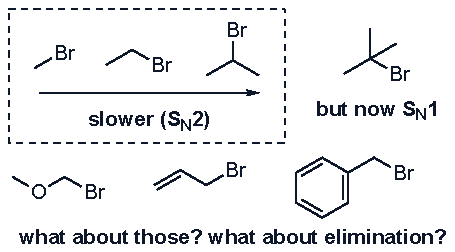
\includegraphics[width=0.7\textwidth]{figures/chapter05-build/model-substrates.pdf}
}

We can now construct the modelling workflow.

\solution{5.0cm}{%
  \centering
  chemical question $\longrightarrow$ define domain $\longrightarrow$ choose response\\[0.6em]
  $\longrightarrow$ assemble or design data $\longrightarrow$ represent chemistry\\[0.6em]
  $\longrightarrow$ fit model $\longrightarrow$ test the claim\\[0.6em]
  $\longrightarrow$ predict $\longrightarrow$ perform the experiment
}

This sequence is not a software pipeline that runs independently of chemistry.
Every arrow contains a chemical decision.
The final arrow is particularly important: a prospective prediction becomes scientifically useful only when the relevant experiment is performed.

% Suggested timing: 5--13 min
\section{What should the model predict?}

An optimisation problem begins with a decision on what the optimisation target is.
Some variables can be represented as continous numbers -- their theoretical range is infinite.
Such \keypoint{continuous variables} can include temperature, time, concentration, pressure, flow rate, and reagent equivalents.
On the other hand, \keypoint{categorical variables} can include solvent, catalyst, ligand, base, or reactor architecture.
The feasible space is smaller than the complete chemical set of all possible combinations because solubility, equipment limits, and chemical compatibility exclude some experiments.
Experimental budget and safety considerations can also drastically reduce the experimental space.

\solution{6cm}
{ \centering
  \textbf{Categorical and continuous variables}
}

The objective defines what counts as improvement.
A reaction with the highest NMR yield may not have the best isolated yield, selectivity, cost, or hazard profile -- it can provide many possible response variables: \textit{e.g.}, rate constant, conversion, yield, regioselectivity, enantioselectivity, product identity.
The objective function therefore encodes priorities rather than revealing a universal optimum.

\begin{figure}[htbp]
  \centering
  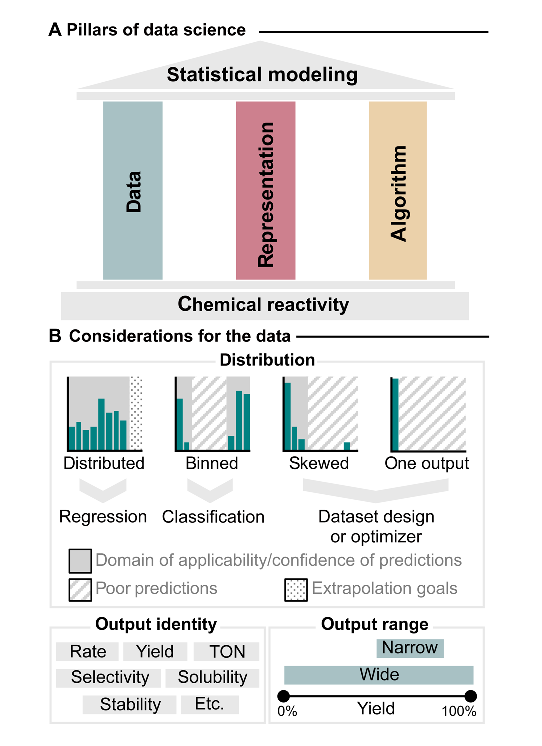
\includegraphics[width=0.6\textwidth]{figures/chapter05-build/07-haas-small-data-modelling-fig1.pdf}
  \caption{Choosing a modelling strategy for sparse chemical data.}
  \label{fig5-haas-small-data}
\end{figure}

Haas, and others emphasise that sparse chemical datasets can contain continuous, binned, skewed, or strongly imbalanced responses, and that the response distribution should influence the statistical strategy.\mcite{Haas2025}
A staged model can sometimes be useful: first classify productive and unproductive reactions, then predict a continuous outcome only for the productive class.

For an asymmetric reaction, percentage enantiomeric excess is intuitive, but its scale is bounded and nonlinear with respect to the free-energy difference between the competing pathways (Fig.~\ref{fig5-ee-ddg}).

\begin{equation}
  \Delta\Delta G^{\ddagger}=-RT\ln\left(\frac{k_{\mathrm{major}}}{k_{\mathrm{minor}}}\right) = -RT \ln\left(\frac{100+ee}{100-ee}\right).
\end{equation}

A difference that looks small in percentage enantiomeric excess near the top of the scale may correspond to a chemically meaningful change in $\Delta\Delta G^{\ddagger}$.
The transformation does not create information, but it places the response on a scale that is more directly connected to the energetic difference between pathways.\mcite{Ruth2024}

\begin{figure}[htbp]
  \centering
  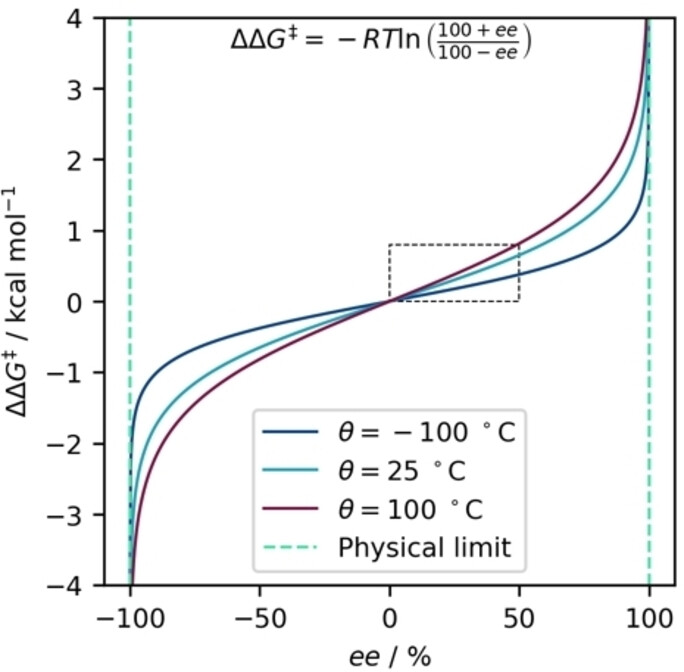
\includegraphics[width=0.45\textwidth]{figures/chapter05-build/ee1.jpg}
  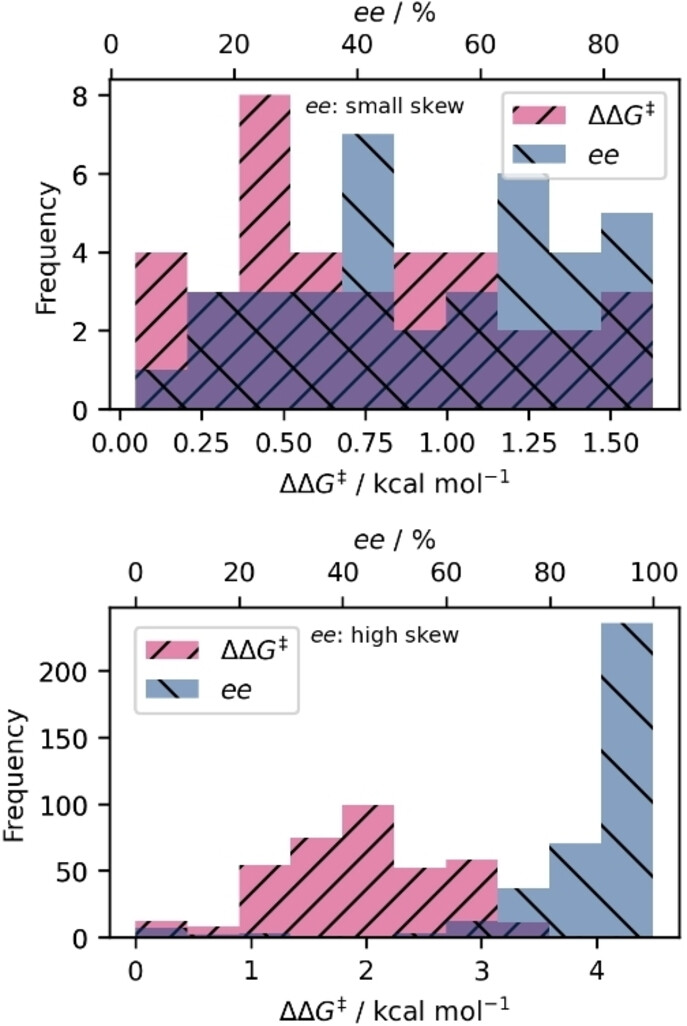
\includegraphics[width=0.45\textwidth]{figures/chapter05-build/ee2.jpg}
  \caption{Difference in response distribution for enantiomeric excess and $\Delta\Delta G^{\ddagger}$.}
  \label{fig5-ee-ddg}
\end{figure}

Dataset design should begin from the intended domain and representation rather than from the data that happen to be convenient.
A literature-derived dataset, a deliberately designed high-throughput campaign, and a conventional reaction scope each provide different distributions of structures, conditions, successes, failures, and measurement uncertainty.
A data-driven modelling project begins by defining the chemical question and domain of applicability, including the reaction space, whether the problem is treated as classification or regression, and the experimental quantity to be predicted. 
Practical constraints then determine what data can realistically be collected: dataset size, high-throughput versus traditional experimentation, and the available analytical methods all influence the achievable scope. 
The dataset itself must then be designed deliberately, choosing appropriate molecular representations and selecting compounds that provide useful coverage of chemical space rather than simply reflecting what is readily available. \mcite{Raghavan2023}
Data acquisition and modelling can also be viewed as an iterative process, in which initial results guide the selection of subsequent experiments, ultimately leading toward active-learning and closed-loop experimental design -- which we will cover at the very end of the course.

\begin{figure}[htbp]
  \centering
  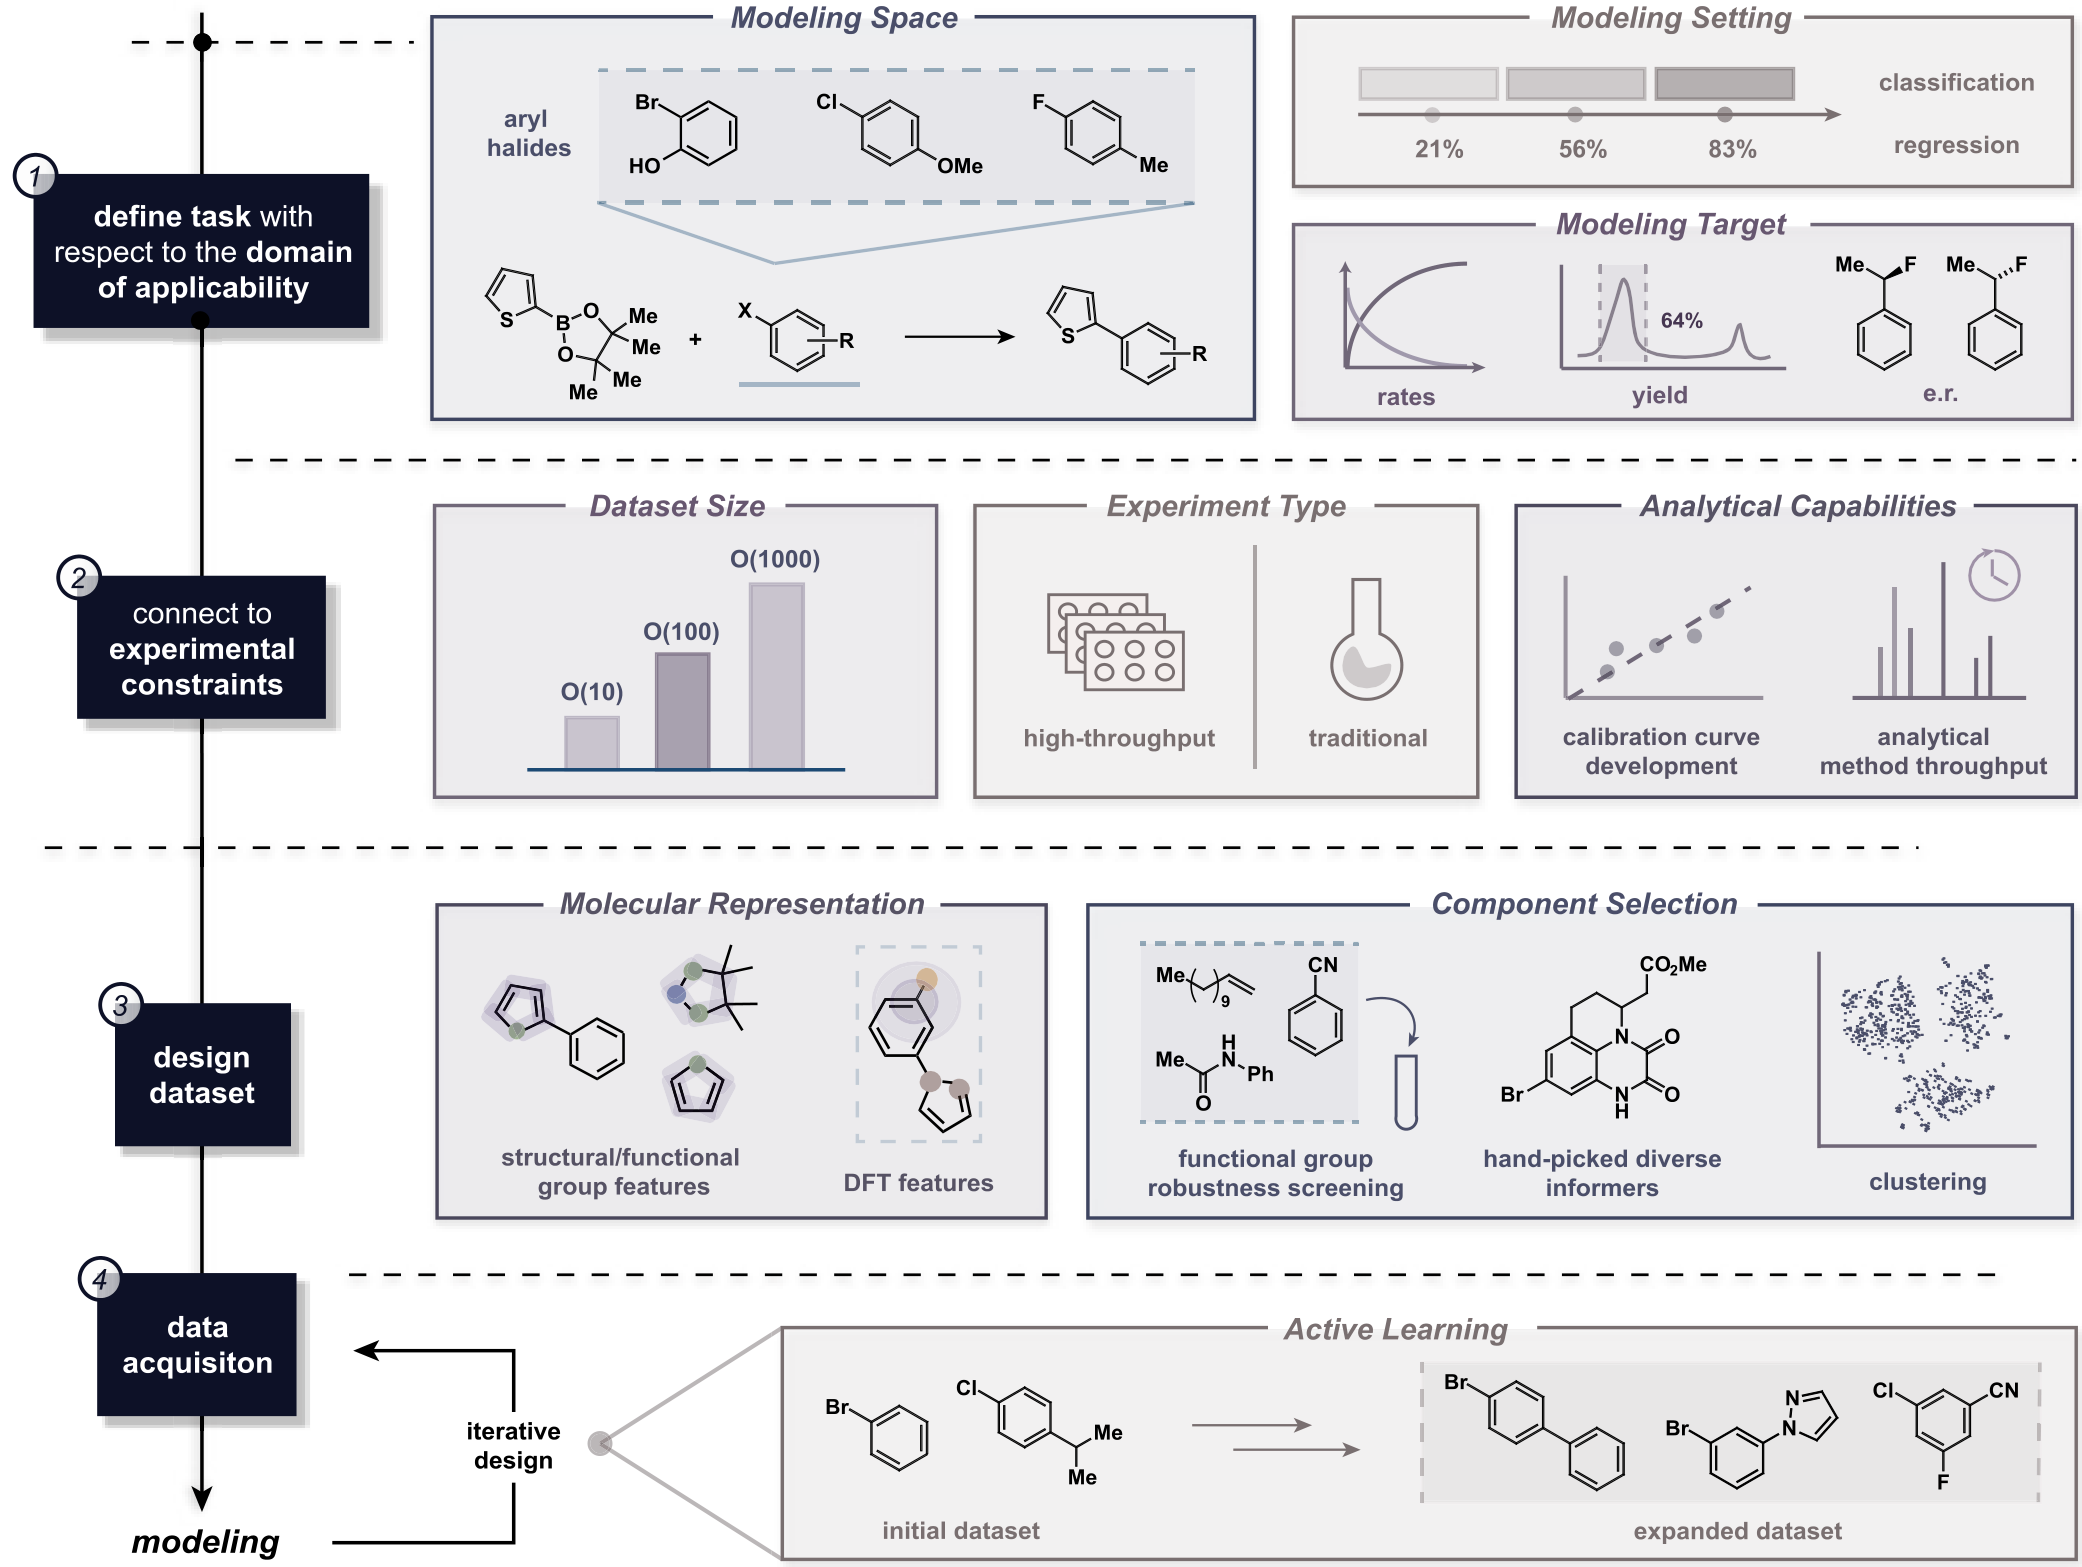
\includegraphics[width=\textwidth]{figures/chapter05-build/01-raghavan-dataset-design-fig1.png}
  \caption{A chemistry-first workflow for dataset design.}
  \label{fig5-raghavan-dataset}
\end{figure}

\solution{8.0cm}{%
  \textbf{Compare two proposed HTE datasets.}\\[0.4em]
  \begin{tabular}{p{0.43\linewidth}p{0.43\linewidth}}
    \textbf{Dataset A} & \textbf{Dataset B}\\
    500 reactions from one narrow ligand family & 40 reactions deliberately spanning steric and electronic space\\
    one substrate class & several substrate classes chosen to test the intended domain\\
    mostly successful literature examples & successful, poor, and failed outcomes recorded consistently
  \end{tabular}\\[0.7em]
}

% Suggested timing: 22--31 min
\section{What information does the model see?}

Chapter~4 represented molecules as points in descriptor space.
A reactivity model connects that representation to a measured response.
The same structure can be encoded using fingerprints, counts of fragments, experimental parameters, calculated physicochemical properties, or descriptors designed around a reactive site.

Return to the selectivity problem.
What might the model need to know about a chiral catalyst?
A SMILES string identifies connectivity, but it does not explicitly state the steric environment around the catalytic pocket.
A single optimised geometry provides three-dimensional information, but a flexible catalyst is an ensemble rather than one frozen structure.

\solution{4.8cm}{%
  \textbf{Possible catalyst information}
  \begin{itemize}
    \item electronic descriptors: charges, orbital energies, electrostatic properties;
    \item steric descriptors: buried volume, Sterimol-type dimensions, spatial occupancy;
    \item conformational descriptors: minima, maxima, ranges, or population-weighted values across an ensemble;
    \item connectivity representations: fingerprints or graph-derived features;
    \item experimental context: substrate identities, solvent, temperature, concentration, and other conditions.
  \end{itemize}
}

Representation, response, and model are separate choices.
A sophisticated algorithm cannot recover information that was never encoded.
Conversely, an expensive descriptor is not automatically useful simply because it required a quantum-chemical calculation.
The relevant question is whether the representation distinguishes the chemistry that controls the response.

Physical-organic chemistry provides the simplest version of this logic.
The Hammett relationship connects a molecular perturbation to a descriptor and then to a response:

\begin{equation}
  \text{structure}\longrightarrow\sigma_{\mathrm{X}}
  \longrightarrow
  \log\left(\frac{k_{\mathrm{X}}}{k_{\mathrm{H}}}\right)=\rho\sigma_{\mathrm{X}}.
\end{equation}

A multivariate linear model extends the same pattern:

\begin{equation}
  y=\beta_0+\beta_1x_1+\beta_2x_2+\cdots+\beta_px_p+\varepsilon.
\end{equation}

The coefficients can be chemically suggestive, but they describe relationships within the sampled data.
Correlated descriptors can exchange apparent importance, and a coefficient does not prove that changing the corresponding molecular property will cause the predicted response.

A flexible nonlinear model may capture relationships that a small linear equation misses.
That can improve prediction, but it can also make the learned relationship more difficult to inspect.
The correct choice depends on the purpose of the model.

\solution{3.8cm}{%
  \textbf{Model A} has the lower test error but is difficult to interpret.\
  \textbf{Model B} predicts slightly less accurately but uses a small number of physically motivated descriptors.\\[0.6em]
  Which is preferable for catalyst ranking? Which is preferable for proposing a mechanistic experiment? Explain why the answer can differ.
}

% Suggested timing: 31--38 min
\section{How do we test the claim?}

A model fitted to every available observation can always be described retrospectively.
The scientific question is whether it predicts data that did not determine its parameters.
We therefore separate model development from final testing.

A random row split is useful when the future use resembles another random row from the same population.
It is much weaker when rows share the same catalysts and substrates in new combinations.
If the intended claim concerns a new catalyst scaffold, a complete catalyst family should be held out.
If it concerns a new substrate class, the relevant substrate family should be held out.

\solution{5.0cm}{%
  \textbf{Draw two validation schemes for a catalyst--substrate matrix.}\\[0.5em]
  \begin{enumerate}
    \item Randomly colour individual cells as training or test reactions.
    \item Hold out an entire row or column corresponding to one catalyst or substrate family.
  \end{enumerate}
  Which scheme tests a claim about unseen experiments? Which tests a stronger claim about unseen chemistry?
}

Training data determine model parameters.
Validation data support choices made during development, such as descriptor selection or hyperparameters.
A test set should be reserved for the final claim.
Repeatedly inspecting the test set while changing the model quietly turns it into another validation set.

Metrics compress model performance into a number, but plots retain chemical structure.
A parity plot can reveal systematic underprediction at high selectivity.
Residuals can reveal that one substrate family is consistently mis-modelled.
A mean absolute error can hide both patterns.

\solution{4.0cm}{%
  \textbf{On a parity plot, annotate:}
  \begin{itemize}
    \item the ideal $y=\hat{y}$ line;
    \item random scatter;
    \item a biased substrate family;
    \item a high-selectivity region containing no training examples.
  \end{itemize}
}

A sensible baseline is also needed.
If a model does not outperform predicting the training-set mean, a simple family average, or a chemically obvious heuristic, its apparent sophistication has not produced a useful relationship.

% Suggested timing: 38--53 min
\section{A complete modelling project: predicting catalyst selectivity}

Zahrt and co-workers provide a useful example because the study connects every stage of the workflow: candidate definition, molecular representation, training-set design, experimental measurement, model fitting, external testing, prediction, and prospective validation.\mcite{Zahrt2019}

\begin{figure}[htbp]
  \centering
  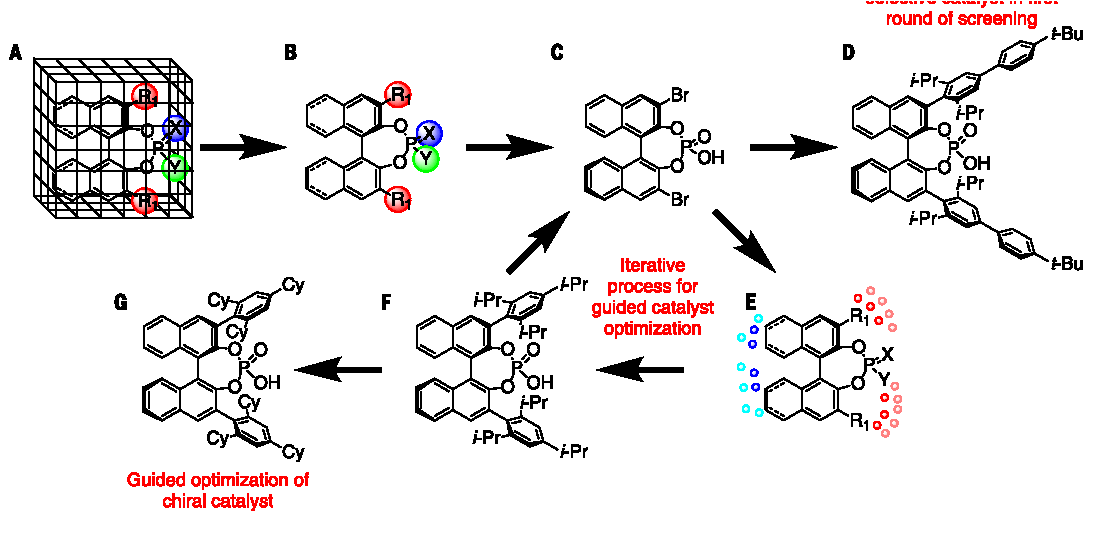
\includegraphics[width=\textwidth,height=0.66\textheight,keepaspectratio]{figures/chapter05-build/02-zahrt-complete-workflow-fig1.pdf}
  \caption{The complete chemoinformatics-guided catalyst workflow: define a virtual catalyst library, calculate descriptors, select a representative subset, measure it, fit the model, and search for improved catalysts. Reproduced from Zahrt \textit{et al.}, \textit{Science} (2019), Fig.~1.}
  \label{fig5-zahrt-workflow}
\end{figure}

\solution{4.6cm}{%
  \textbf{Build the workflow on the figure one panel at a time.}
  \begin{itemize}
    \item Number the panels as domain, representation, sampling, experiment, model, prediction, and prospective test.
    \item Put a star beside the first panel that uses measured selectivity.
    \item Draw a box around the stages that can be completed before any catalyst is synthesised.
    \item Write the chemical claim tested by the final experiment.
  \end{itemize}
}

\subsection{Define the catalyst domain}

The authors did not begin from a short list of familiar catalysts.
They generated a virtual library of 403 synthetically feasible chiral phosphoric-acid catalysts across two related scaffolds.
The purpose of the virtual library was not to claim that every structure would be equally easy to make.
It was to define a candidate domain before experimental selection.

\solution{2.8cm}{%
  \textbf{Question before revealing the workflow:} If only a small number of catalysts can be tested, should they be selected at random, selected from familiar examples, or selected to cover the calculated catalyst space?
}

\subsection{Represent the catalyst as an ensemble}

The catalysts were represented using rapidly calculated, conformer-aware descriptors.
The average steric occupancy representation retains three-dimensional information from the catalyst conformational ensemble rather than treating a single minimum-energy geometry as the whole molecule.
This matters because different accessible conformers can present different steric environments to the reacting substrates.

The descriptor calculation maps each candidate catalyst to a point in a common property space.
That makes a representative selection possible before selectivity has been measured.

\subsection{Choose a universal training set}

A representative 24-catalyst universal training set was selected from the virtual catalyst space.
It was called ``universal'' because the selection used catalyst properties rather than the outcome of one particular reaction.
This is the connection to Chapter~4: representative selection covers a chosen representation without yet knowing the response.

\begin{figure}[htbp]
  \centering
  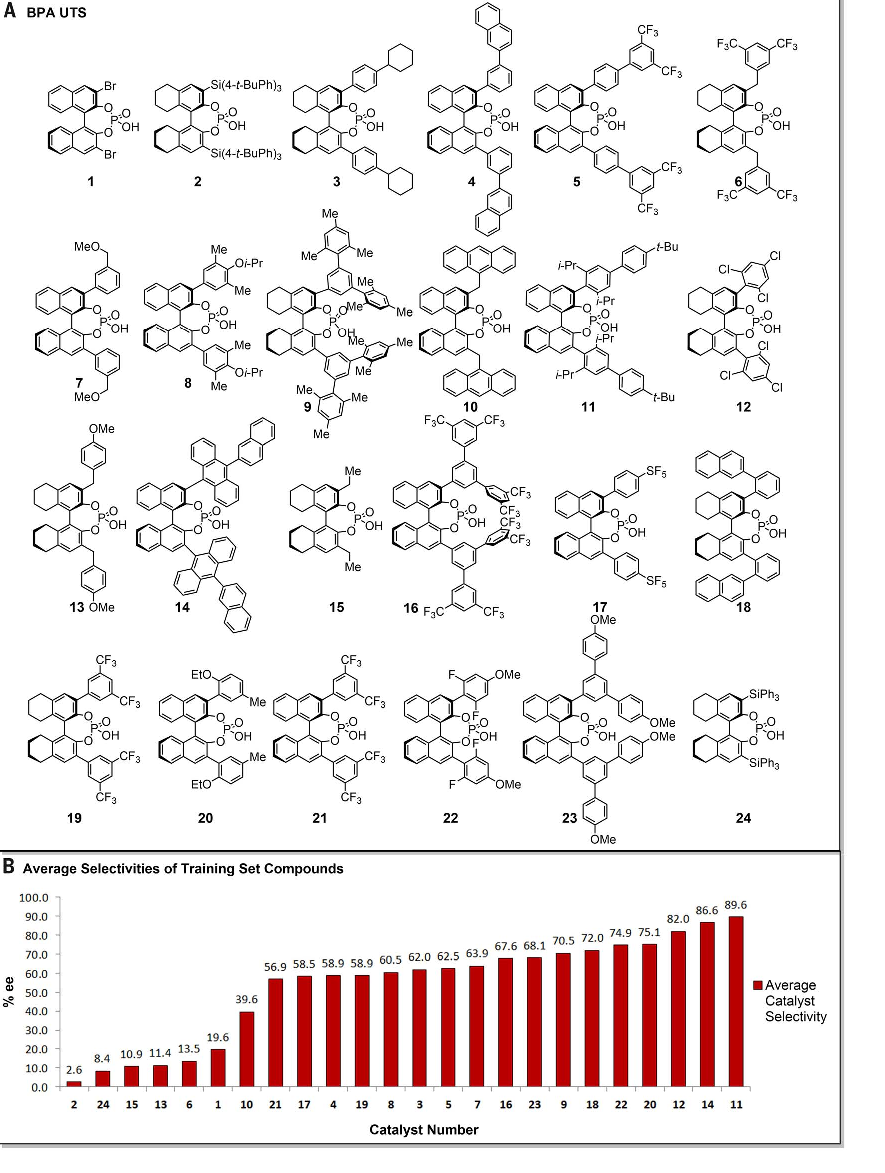
\includegraphics[width=\textwidth,height=0.70\textheight,keepaspectratio]{figures/chapter05-build/03-zahrt-universal-training-set-fig4.pdf}
  \caption{The selected phosphoric-acid catalyst training set and its measured selectivity across the training reactions. The figure makes the transition from descriptor-space coverage to experimental response visible. Reproduced from Zahrt \textit{et al.}, \textit{Science} (2019), Fig.~4.}
  \label{fig5-zahrt-uts}
\end{figure}

\solution{3.8cm}{%
  \textbf{Annotate the existing catalyst-space figure.}
  \begin{itemize}
    \item circle the 24 training catalysts;
    \item mark a candidate surrounded by training examples;
    \item mark a candidate in a poorly covered region;
    \item state which prediction is more clearly interpolative in this representation.
  \end{itemize}
}

\subsection{Collect the experimental responses}

The study examined 43 catalysts in total: the 24 training catalysts and 19 external catalysts.
Each catalyst was tested across 25 products formed from pairwise combinations of imines and thiols.
Duplicate measurements gave 2150 experiments in total.
The repeated catalyst--substrate matrix allowed the model to learn from systematic variation rather than from unrelated reaction records.

At this point, the abstract symbols acquire chemical meaning:

\solution{4.0cm}{%
  \begin{equation}\begin{aligned}
    \text{one row} & = \text{one catalyst--imine--thiol combination},\\
    \mathbf{X} & = \text{catalyst and substrate descriptors},\\
    y & = \Delta\Delta G^{\ddagger}\text{ derived from selectivity},\\
    f(\mathbf{X}) & = \text{the fitted structure--selectivity relationship}.
  \end{aligned}\end{equation}
}

\subsection{Test several kinds of novelty}

The authors did not rely on one random split.
They tested new substrate combinations, external catalysts, and combinations in which both catalyst and product were outside the corresponding training combinations.
Those tests are chemically different even when they contain similar numbers of rows.

The model also predicted reactions with selectivities higher than those used for training.
This is response-range extrapolation.
It should not be confused with extrapolation to an unrepresented catalyst family.
A predicted response can lie beyond the observed $y$ range while the catalyst remains in a well-covered region of descriptor space.
Conversely, a response can fall inside the training range for a chemically remote catalyst.

\solution{3.8cm}{%
  \textbf{Classify each proposed prediction.}
  \begin{enumerate}
    \item familiar catalyst region, but selectivity above the observed training range;
    \item unfamiliar catalyst scaffold, but selectivity inside the observed range;
    \item new catalyst--substrate combination assembled from familiar components.
  \end{enumerate}
  Which involves response extrapolation? Which involves representation or component extrapolation?
}

\subsection{Close the loop with experiment}

After validation, the model was used to search the larger virtual library and identify promising catalysts.
The predicted catalysts were then synthesised and tested.
This prospective experiment is the part that converts a modelling exercise into a catalyst-discovery workflow.

Return to Figs.~\ref{fig5-zahrt-workflow} and \ref{fig5-zahrt-uts}. The first is the project architecture; the second shows what the selected training catalysts actually did. The workflow is only coherent if the sampling decision, experimental matrix, validation claim, and prospective test refer to the same chemical domain.

\solution{5.2cm}{%
  \textbf{Complete the evidence chain across the two Zahrt figures.}
  \begin{itemize}
    \item On Fig.~\ref{fig5-zahrt-workflow}, write the modelling decision above each panel.
    \item On Fig.~\ref{fig5-zahrt-uts}, circle the 24 training catalysts and mark where the response first becomes visible.
    \item Mark one catalyst prediction that is interpolative in descriptor space and one that would be less well supported.
    \item Finish the sentence: ``The prospective experiment is stronger than another random test row because \ldots''
  \end{itemize}
}

\begin{conceptbox}
  \keypoint{The model is credible because the whole workflow is aligned.}
  The candidate domain is explicit, the training catalysts cover a chosen representation, the response is measured systematically, novelty is tested in several ways, and the final prediction is checked experimentally.
\end{conceptbox}

% Suggested timing: 53--58 min
\section{A contrasting model: nonlinear prediction across catalyst families}

Singh and co-workers assembled asymmetric-hydrogenation data spanning five families of chiral catalysts and represented catalysts and substrates using quantum-derived descriptors.\mcite{Singh2020}
Random-forest models captured nonlinear relationships that would be difficult to express with a small linear equation.
The case is useful because it separates three ideas that are often bundled together: descriptor sophistication, algorithm flexibility, and chemical generalisation.

\begin{figure}[htbp]
  \centering
  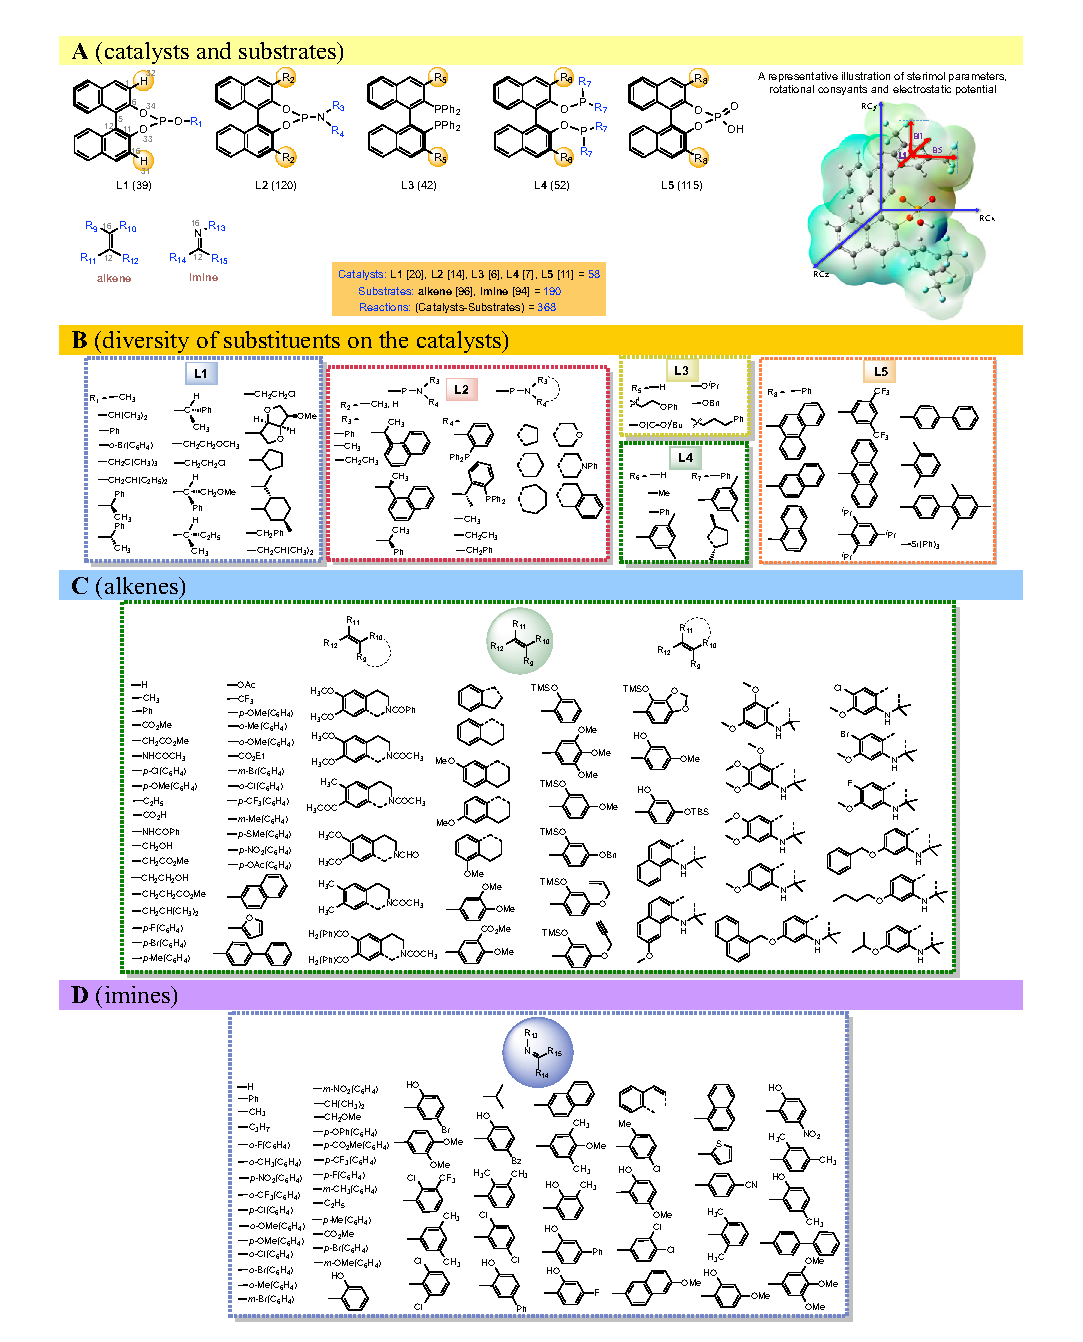
\includegraphics[width=\textwidth,height=0.70\textheight,keepaspectratio]{figures/chapter05-build/04-singh-catalyst-substrate-domain-fig1.pdf}
  \caption{Catalyst and substrate families used to construct a unified asymmetric-hydrogenation model, together with representative molecular descriptors. Reproduced from Singh \textit{et al.}, \textit{PNAS} (2020), Fig.~1.}
  \label{fig5-singh-domain}
\end{figure}

\solution{3.8cm}{%
  \textbf{Define the domain before looking at performance.}
  \begin{itemize}
    \item Bracket each catalyst family and write how many chemically distinct families the model must join.
    \item Circle the substrate features that can vary independently of catalyst identity.
    \item Predict which held-out family would be the strongest test of transfer, and state why.
  \end{itemize}
}

Performance decreased as the external test chemistry became more distinct from the catalyst families represented during training.
Chemical novelty is therefore graded rather than binary.
A catalyst can be unlike its nearest training examples in some descriptors but not others, and the relevant distance depends on whether those descriptors encode the chemistry controlling the response.

\begin{figure}[htbp]
  \centering
  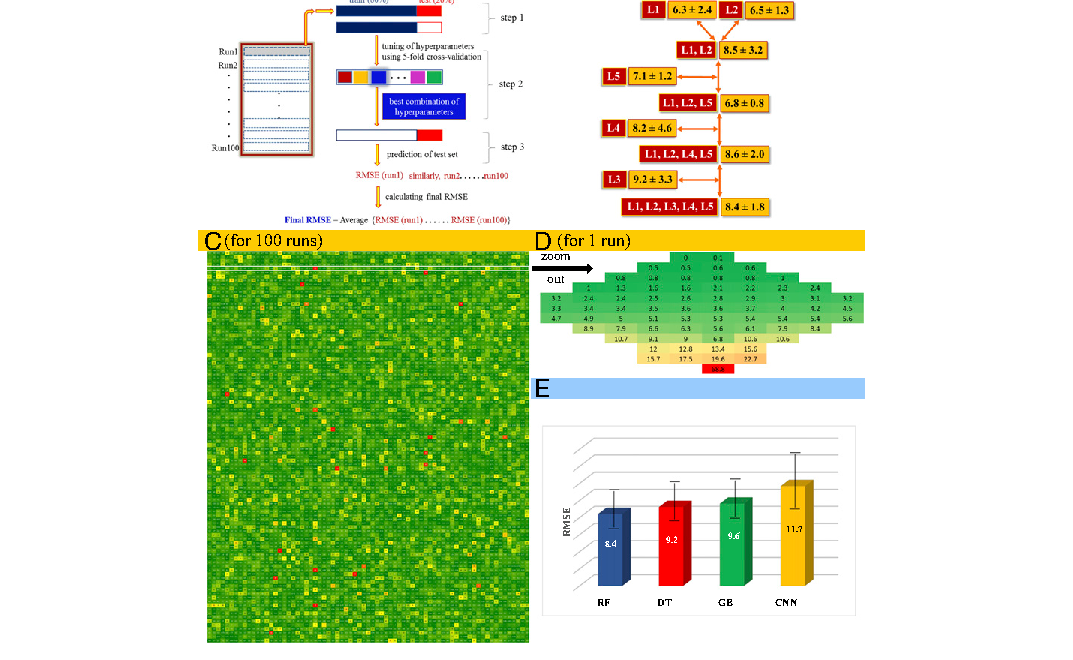
\includegraphics[width=\textwidth,height=0.66\textheight,keepaspectratio]{figures/chapter05-build/05-singh-unified-random-forest-fig2.pdf}
  \caption{Unified random-forest validation across catalyst--substrate subsets. Aggregate error and subgroup behaviour must be read together. Reproduced from Singh \textit{et al.}, \textit{PNAS} (2020), Fig.~2.}
  \label{fig5-singh-rf}
\end{figure}

\solution{4.2cm}{%
  \textbf{Read performance chemically, not only numerically.}
  \begin{itemize}
    \item Identify the subsets with the smallest and largest errors.
    \item Mark where an overall RMSE would conceal family-dependent performance.
    \item Write beside one subgroup whether it is interpolation, recombination of familiar components, or transfer to a new family.
  \end{itemize}
}

The authors also used a decision tree to identify descriptor combinations associated with high predicted selectivity.
Those branches generate chemical hypotheses about useful combinations of catalyst and substrate properties.
They do not, by themselves, identify causal transition-state interactions.
That distinction is the starting point for Chapter~6.

\begin{figure}[htbp]
  \centering
  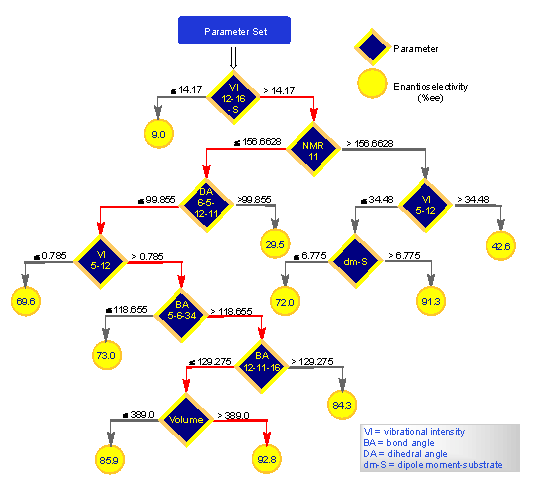
\includegraphics[width=\textwidth,height=0.55\textheight,keepaspectratio]{figures/chapter05-build/06-singh-decision-tree-fig4.pdf}
  \caption{Decision-tree analysis linking combinations of catalyst and substrate descriptors to promising selectivity regimes. The branches are predictive rules, not a mechanistic proof. Reproduced from Singh \textit{et al.}, \textit{PNAS} (2020), Fig.~4.}
  \label{fig5-singh-tree}
\end{figure}

\solution{3.8cm}{%
  \textbf{Turn one branch into a testable chemical hypothesis.}
  \begin{itemize}
    \item Trace one red path from the root to a high-selectivity leaf.
    \item Translate each numerical split into a statement about catalyst or substrate structure.
    \item Add one independent experiment that could test whether the highlighted descriptor is causal or merely correlated.
  \end{itemize}
}

\solution{3.2cm}{%
  \textbf{Compare the Zahrt and Singh workflows.}
  \begin{itemize}
    \item Where does deliberate chemical-space selection enter?
    \item Which representations are conformer- or quantum-informed?
    \item What kind of external chemistry is used for testing?
    \item Which conclusions are predictive, and which would require independent mechanistic evidence?
  \end{itemize}
}

% Suggested timing: 58--60 min
\section{A modelling-project checklist}

Before accepting a chemical modelling project, ask:

\solution{5.0cm}{%
  \begin{enumerate}
    \item \textbf{Question:} What exact decision or scientific claim is the model intended to support?
    \item \textbf{Domain:} Which catalyst, substrate, reagent, and condition families are included?
    \item \textbf{Response:} What is measured, in which units, and with what uncertainty?
    \item \textbf{Observations:} What does one row mean, and how were rows selected?
    \item \textbf{Representation:} Which chemical information is visible to the model, and what is omitted?
    \item \textbf{Model:} Is the complexity justified by the amount and structure of the data?
    \item \textbf{Test:} Does the split reproduce the chemical novelty claimed for future use?
    \item \textbf{Experiment:} Has a prospective prediction actually been tested?
  \end{enumerate}
}

\section{Summary}

A chemical modelling project begins with a defined question, domain, and response rather than an algorithm.
The dataset determines which chemistry the model can learn, while the representation determines which distinctions are visible.
Regression and classification should follow the chemical response and its distribution.
Validation must reproduce the novelty implied by the scientific claim; an unseen row is not necessarily unseen chemistry.
The Zahrt study shows how virtual-library design, conformer-aware descriptors, representative training-set selection, systematic experimentation, external testing, and prospective validation can form one coherent catalyst-discovery workflow.
The Singh study shows both the value of flexible nonlinear models and the continuing limitation imposed by chemical distance from the training domain.
Chapter~6 now asks the harder question: when a model makes a prediction or highlights a descriptor, what should we believe, and what chemistry can we learn from it?
